%%%%%%%%%%%%%%%%%%%%%%%%%%%%%%%%%%%%%%%%%%%%%%%%%%%%%%%%%%%%%%%%%%
%%%%%%%% BENELEARN 2013 EXAMPLE LATEX SUBMISSION FILE %%%%%%%%%%%%%%%%%
%%%%%%%%%%%%%%%%%%%%%%%%%%%%%%%%%%%%%%%%%%%%%%%%%%%%%%%%%%%%%%%%%%

% Use the following line _only_ if you're still using LaTeX 2.09.
%\documentstyle[benelearn2012,epsf,mlapa]{article}
% If you rely on Latex2e packages, like most moden people use this:
\documentclass{article}

% Employ the following version of the ``usepackage'' statement for
% submitting the draft version of the paper for review.  This will set
% the note in the first column to ``Under review.  Do not distribute.''

\usepackage{benelearn2013}

% Employ this version of the ``usepackage'' statement after the paper has
% been accepted, when creating the final version.  This will set the
% note in the first column to ``Appearing in''
%\usepackage[accepted]{benelearn2013}

% For figures
\usepackage{graphicx} % more modern
%\usepackage{epsfig} % less modern
\usepackage{subfigure}

% For citations
\usepackage{mlapa}

% The \benelearntitle you define below is probably too long as a header.
% Therefore, a short form for the running title is supplied here:
\benelearntitlerunning{Formatting Instructions for BENELEARN 2013 Papers}

\begin{document}

\twocolumn[
\benelearntitle{Formatting Instructions for BENELEARN 2013 Papers \\
           \texttt{http://www.benelearn2013.org/}}

 \benelearnauthor{Your Name}{email@yourdomain.edu}
 \benelearnaddress{Your Fantastic Institute,
             van Goghstraat 7, 2387, Baarle-Hertog, Belgium}
 \benelearnauthor{Your CoAuthor's Name}{email@coauthordomain.edu}
 \benelearnaddress{Their Fantastic Institute,
             Magrittelaan 42, 5110 AB Baarle-Nassau, The Netherlands}
\benelearnaddress{{\bf Keywords}: submission information, deadline data,
	formatting information
          }
\vskip 0.3in
]

\begin{abstract}

In the following, you will find formatting guidelines for the submission of a BENELEARN 2013 long paper.  

\end{abstract}

\section{Electronic Submission}
\label{submission}

\subsection{Templates for Papers}

Electronic templates for producing papers for submission are available for \LaTeX\/ at the BENELEARN website.

If you are using the templates, the formatting instructions below will already be enforced. The content rules you must follow are:
\begin{itemize}
\item The maximum paper length for full papers is 8 pages (references included).  For abstracts, it is 1 page.
\item You are allowed to include author information or acknowledgments in your initial submission. The review process will be single blind. Do include keywords.
\item Place figure captions {\em under} the figure (and omit titles from inside the graphic file itself). Place table captions {\em over} the table.
\item References must include page numbers whenever possible and be as complete as possible. Place multiple citations in chronological order.
\end{itemize}
Please see below for details on each of these items.

\subsection{Submitting Papers}

Submission to BENELEARN will be entirely electronic, by means of easychair (follow the link on the website).  

{\bf Paper Deadline:} The deadline for paper submission to BENELEARN 2013 is March 12th, 2013.

To ensure our ability to print submissions, authors must provide their manuscripts in \textbf{PDF} format. Furthermore, please make sure that files contain only Type-1 fonts (e.g.,~using the program {\tt pdffonts} in linux or using File/DocumentProperties/Fonts in Acrobat).  Other fonts (like Type-3) might come from graphics files imported into the document.

Authors should pay close attention to the \textbf{\LaTeX} typefaces used.  Specifically, when converting the dvi output of \LaTeX to Postscript the default behavior is to use non-scalable Type-3 PostScript bitmap fonts to represent the standard \LaTeX fonts. The resulting document is difficult to read in electronic form; the type appears fuzzy. To avoid this problem, dvips must be instructed to use an alternative font map.  This can be achieved with something like the following commands:\\ {\bf dvips -Ppdf -tletter -G0 -o paper.ps paper.dvi}\\ {\bf ps2pdf paper.ps}\\ Note that it is a zero following the ``-G''. This tells dvips to use the config.pdf file (and this file refers to a better font mapping).

Another alternative is to use the \textbf{pdflatex} program instead of straight \LaTeX. This program avoids the Type-3 font problem, however you must ensure that all of the fonts are embedded (use {\tt pdffonts}). If they are not, you need to configure pdflatex to use a font map file that specifies that the fonts be embedded. Also you should ensure that images are not downsampled or otherwise compressed in a lossy way.

\subsection{Submitting Final Camera-Ready Copy}

The final versions of papers accepted for publication should follow the same format and naming convention as initial submissions. See Section~\ref{final author} for details of how to format this.

The footnote, ``Preliminary work.  Under review by the annual machine learning conference of Belgium and The Netherlands (BENELEARN). Do not distribute.'' must be
modified to ``Appearing in \textit{Proceedings of BENELEARN 2013}. Copyright 2013 by the author(s)/owner(s).'' In your .tex file, simply change
$\mathtt{\backslash usepackage\{benelearn2013\}}$ to $\mathtt{\backslash
usepackage[accepted]\{benelearn2013\}}$.  

Camera-ready copies should have the title of the paper as running head on each page except the first one.  The running title consists of a single line centered above a horizontal rule which is $1$ point thick. The running head should be centered, bold and in $9$ point type.  The rule should be $10$ points above the main text.  For the camera-ready copies, the original title is automatically set as running head using the {\tt fancyhdr} package which can be obtained at the BENELEARN 2013 web site. In cases where the original title exceeds the size restrictions, a shorter form can be supplied by using
$$\mathtt{\backslash benelearntitlerunning\{\ldots\}}$$
just before $\mathtt{\backslash begin\{document\}}$.

\section{Format of the Paper}

All submissions should follow the same format to ensure the printer can reproduce them without problems and to let readers more easily find the information that they desire.

\subsection{Length and Dimensions}

Papers must not exceed 8 pages (1 page for abstracts).
including all figures, tables, references, and appendices. We will return to the authors any submissions that exceed this page limit or that diverge significantly from the format specified herein.

The text of the paper should be formatted in two columns, with an overall width of 6.75 inches, height of 9.0 inches, and 0.25 inches between the columns. The left margin should be 0.75 inches and the top margin 1.0 inch (2.54~cm). The right and bottom margins will depend on whether you print on US letter or A4 paper, but all final versions must be produced for A4 paper.

The paper body should be set in 10~point type with a vertical spacing of 11~points. Please use Times Roman typeface throughout the text.

\subsection{Title}

The paper title should be set in 14~point bold type and centered between two horizontal rules that are 1~point thick, with 1.0~inch between the top rule and the top edge of the page. Capitalize the first letter of content words and put the rest of the title in lower case.


\subsubsection{Author Information}
\label{final author}
The review process will be single blind. Author information should start 0.3~inches below the bottom rule surrounding the title. The authors' names should appear in 10~point bold type, electronic mail addresses in 10~point small capitals, and physical addresses in ordinary 10~point type. Each author's name should be flush left, whereas the email address should be flush right on the same line. The author's physical address should appear flush left on the ensuing line, on a single line if possible. If successive authors have the same affiliation, then give their physical address only once.

\subsection{Abstract}

The paper abstract should begin in the left column, 0.4~inches below the final address. The heading `Abstract' should be centered, bold, and in 11~point type. The abstract body should use 10~point type, with a vertical spacing of 11~points, and should be indented 0.25~inches more than normal on left-hand and right-hand margins. Insert 0.4~inches of blank space after the body. Keep your abstract brief, limiting it to one paragraph and no more than six or seven sentences.

\subsubsection{Sections and Subsections}

Section headings should be numbered, flush left, and set in 11~pt bold type with the content words capitalized. Leave 0.25~inches of space before the heading and 0.15~inches after the heading.

Similarly, subsection headings should be numbered, flush left, and set in 10~pt bold type with the content words capitalized. Leave 0.2~inches of space before the heading and 0.13~inches afterward.

Finally, subsubsection headings should be numbered, flush left, and set in 10~pt small caps with the content words capitalized. Leave 0.18~inches of space before the heading and 0.1~inches after the heading. Please use no more than three levels of headings.

\subsubsection{Paragraphs and Footnotes}

Within each section or subsection, you should further partition the paper into paragraphs. Do not indent the first line of a given paragraph, but insert a blank line between succeeding ones.

You can use footnotes\footnote{For the sake of readability, footnotes should be complete sentences.} to provide readers with additional information about a topic without interrupting the flow of the paper. Indicate footnotes with a number in the text where the point is most relevant. Place the footnote in 9~point type at the bottom of the column in which it appears. Precede the first footnote in a column with a horizontal rule of 0.8~inches.\footnote{Multiple footnotes can appear in each column, in the same order as they appear in the text, but spread them across columns and pages if possible.}

\begin{figure}[ht]
\vskip 0.2in
\begin{center}
\centerline{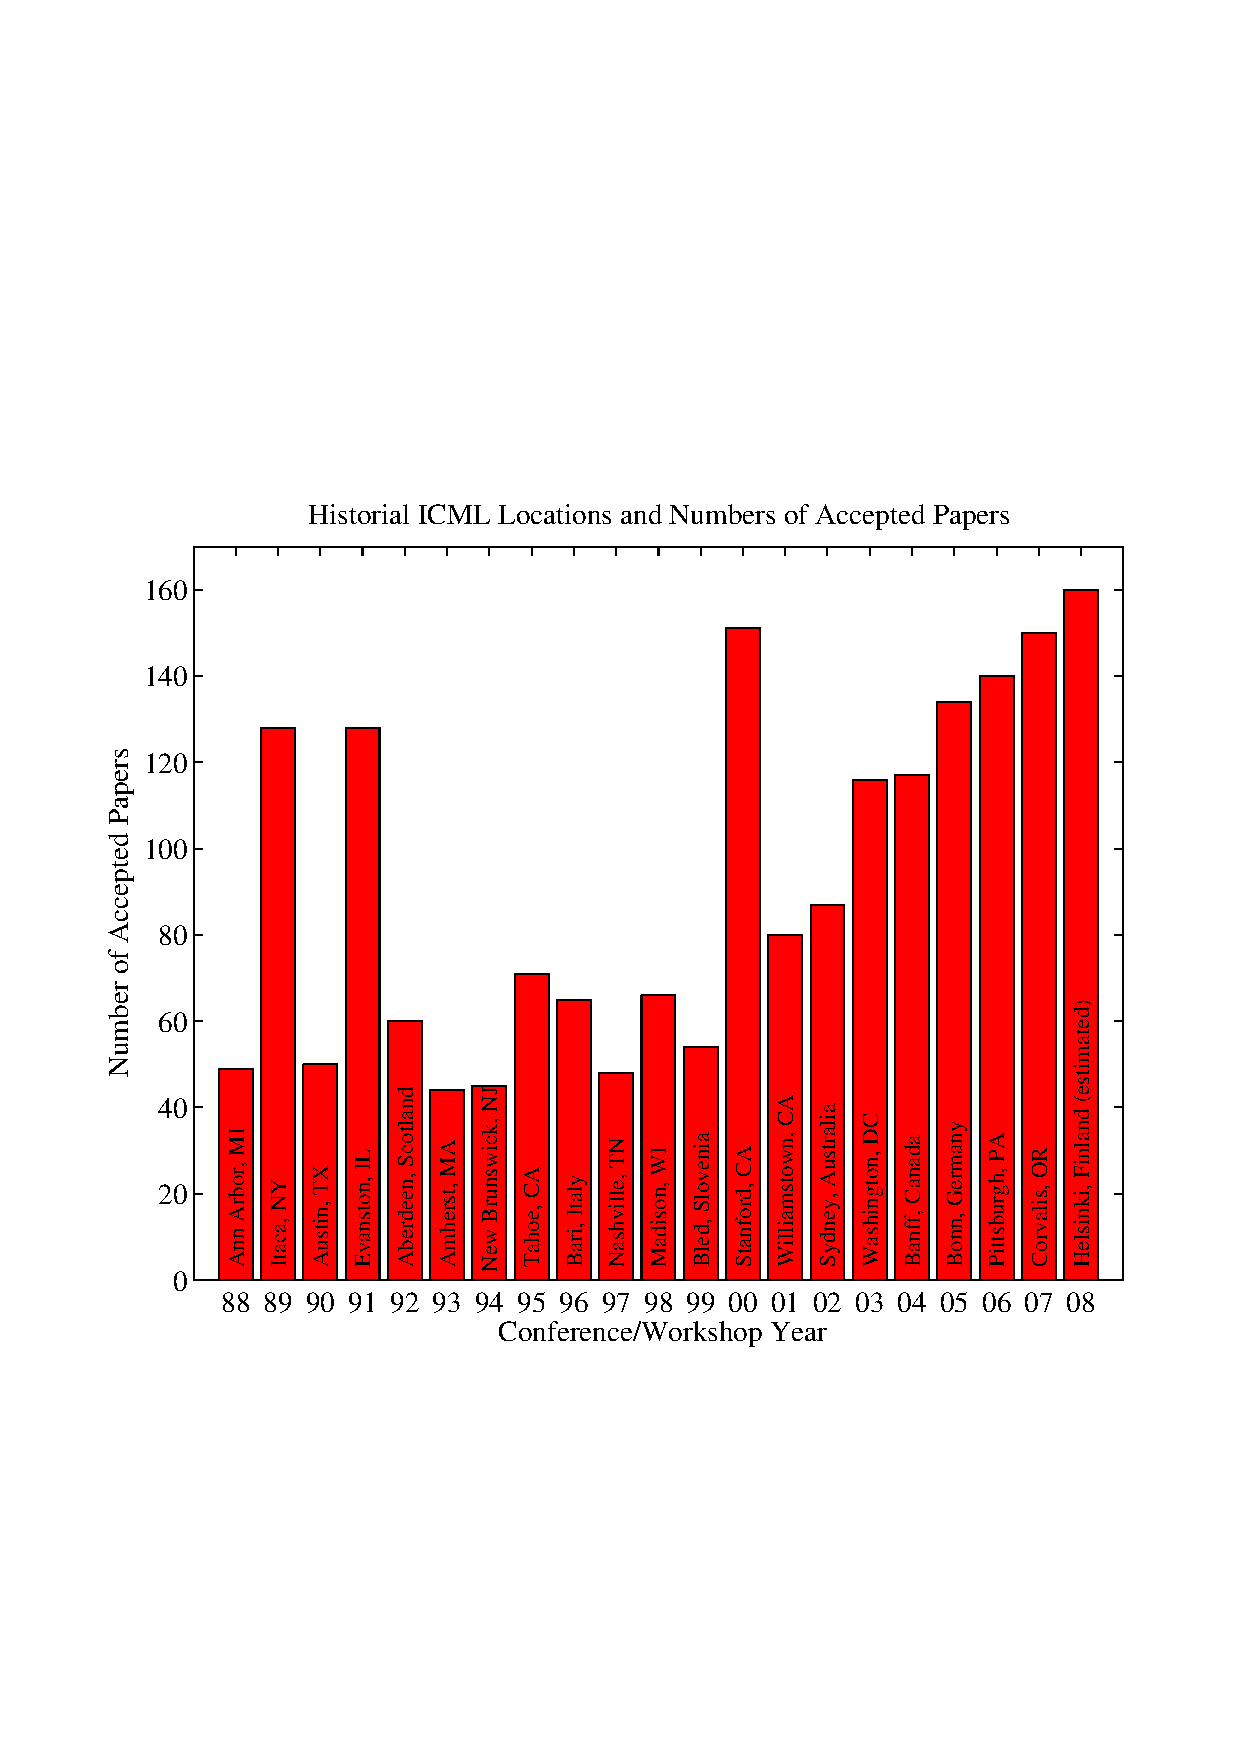
\includegraphics[width=\columnwidth]{icml_numpapers}}
\caption{Historical locations and number of accepted papers for International
  Machine Learning Conferences (ICML 1993 -- ICML 2008) and
  International Workshops on Machine Learning (ML 1988 -- ML
  1992). At the time this figure was produced, the number of
  accepted papers for ICML 2008 was unknown and instead estimated.}
\label{icml-historical}
\end{center}
\vskip -0.2in
\end{figure}

\subsection{Figures}

You may want to include figures in the paper to help readers visualize your approach and your results. Such artwork should be centered, legible, and separated from the text. Lines should be dark and at least 0.5~points thick for purposes of reproduction, and text should not appear on a gray background.

Label all distinct components of each figure. If the figure takes the form of a graph, then give a name for each axis and include a legend that briefly describes each curve. Do not include a title inside the figure; instead, the caption should serve this function.

Number figures sequentially, placing the figure number and caption {\it after\/} the graphics, with at least 0.1~inches of space before the caption and 0.1~inches after it, as in
Figure~\ref{icml-historical}.  The figure caption should be set in 9~point type and centered unless it runs two or more lines, in which case it should be flush left.  You may float figures to the top or bottom of a column, and you may set wide figures across both columns (use the environment {\tt figure*}), but always place two-column figures at the top or bottom of the page.

\subsection{Algorithms}

Please use the ``algorithm'' and ``algorithmic''
environments to format pseudocode in \LaTeX\/. These require
the corresponding stylefiles, algorithm.sty and
algorithmic.sty, which are supplied with this package.
Algorithm~\ref{alg:example} shows an example.

\begin{algorithm}[tb]
   \caption{Bubble Sort}
   \label{alg:example}
\begin{algorithmic}
   \STATE {\bfseries Input:} data $x_i$, size $m$
   \REPEAT
   \STATE Initialize $noChange = true$.
   \FOR{$i=1$ {\bfseries to} $m-1$}
   \IF{$x_i > x_{i+1}$}
   \STATE Swap $x_i$ and $x_{i+1}$
   \STATE $noChange = false$
   \ENDIF
   \ENDFOR
   \UNTIL{$noChange$ is $true$}
\end{algorithmic}
\end{algorithm}

\subsection{Tables}

You may also want to include tables that summarize material. Like figures, these should be centered, legible, and numbered consecutively. However, place the title {\it above\/} the table with at least 0.1~inches of space before the title and the same after it, as in Table~\ref{sample-table}. The table title should be set in 9~point type and centered unless it runs two or more lines, in which case it should be flush left.

% Note use of \abovespace and \belowspace to get reasonable spacing
% above and below tabular lines.

\begin{table}[t]
\caption{Classification accuracies for naive Bayes and flexible
Bayes on various data sets.}
\label{sample-table}
\vskip 0.15in
\begin{center}
\begin{small}
\begin{sc}
\begin{tabular}{lcccr}
\hline
\abovespace\belowspace
Data set & Naive & Flexible & Better? \\
\hline
\abovespace
Breast    & 95.9$\pm$ 0.2& 96.7$\pm$ 0.2& $\surd$ \\
Cleveland & 83.3$\pm$ 0.6& 80.0$\pm$ 0.6& $\times$\\
Glass2    & 61.9$\pm$ 1.4& 83.8$\pm$ 0.7& $\surd$ \\
Credit    & 74.8$\pm$ 0.5& 78.3$\pm$ 0.6&         \\
Horse     & 73.3$\pm$ 0.9& 69.7$\pm$ 1.0& $\times$\\
Meta      & 67.1$\pm$ 0.6& 76.5$\pm$ 0.5& $\surd$ \\
Pima      & 75.1$\pm$ 0.6& 73.9$\pm$ 0.5&         \\
\belowspace
Vehicle   & 44.9$\pm$ 0.6& 61.5$\pm$ 0.4& $\surd$ \\
\hline
\end{tabular}
\end{sc}
\end{small}
\end{center}
\vskip -0.1in
\end{table}

Tables contain textual material that can be typeset, as contrasted with figures, which contain graphical material that must be drawn. Specify the contents of each row and column in the table's topmost row. Again, you may float tables to a column's top or bottom, and set wide tables across both columns, but place two-column tables at the top or bottom of the page.

\subsection{Citations and References}
Please use APA reference format. Within the \LaTeX\/ bibliographic facility, use {\tt mlapa.sty} and {\tt mlapa.bst} to obtain this format.

Citations within the text should include the authors' last names and year. If the authors' names are included in the sentence, place only the year in parentheses, for example when referencing Rob Schapire's seminal result \yrcite{schapire90}. Otherwise place the entire reference in parentheses with the authors and year separated by a comma \cite{schapire90}.

List multiple references separated by semicolons \cite{kearns89,schapire90,neal93}. Use the `et~al.' construct only for citations with four or more authors or after listing all authors to a publication in an earlier reference.

Use an unnumbered first-level section heading for the references, and use a hanging indent style, with the first line of the reference flush against the left margin and subsequent lines indented by 10 points. The references at the end of this document give examples for journal articles, conference publications, book chapters, books, edited volumes,
technical reports, and dissertations.

Alphabetize references by the surnames of the first authors, with single author entries preceding multiple author entries. Order references for the same authors by year of publication, with the earliest first.

\section*{Acknowledgments}
If a paper is accepted, the final camera-ready version can (and
probably should) include acknowledgements. In this case, please place such acknowledgements in an unnumbered section at the end of the paper. Typically, this will include thanks to reviewers who gave useful comments, to colleagues who contributed to the ideas, and to funding agencies and corporate sponsors that provided financial support.

% In the unusual situation where you want a paper to appear in the
% references without citing it in the main text, use \nocite
\nocite{zinkevich03}

\bibliography{example_paper}
\bibliographystyle{mlapa}

\end{document}

% Version History
% Document updated by Florian Kunneman for BENELEARN 2013
% Document updated by Willem Waegeman for BeneLearn 2012
% Document updated by Peter van der Putten for BeneLearn 2011
% This document was modified by Kurt Driessens for BeneLearn 2010.
% Before it was modified from the file originally made available by
% Pat Langley and Andrea Danyluk for ICML-2K. This 2009 version was
% created by Kiri Wagstaff, slightly modified from Sam Roweis's 2008
% version, which is slightly modified from Prasad Tadepalli's 2007
% version which is a lightly changed version of the previous year's
% version by Andrew Moore, which was in turn edited from those of
% Kristian Kersting and Codrina Lauth. Alex Smola contributed to the
% algorithmic style files.


